% !TEX program = XeLaTeX
% !TEX encoding = UTF-8
\documentclass[UTF8,nofonts]{ctexart}
\setCJKmainfont[BoldFont=FandolSong-Bold.otf,ItalicFont=FandolKai-Regular.otf]{FandolSong-Regular.otf}
\setCJKsansfont[BoldFont=FandolHei-Bold.otf]{FandolHei-Regular.otf}
\setCJKmonofont{FandolFang-Regular.otf}

\usepackage{url}
\usepackage{cancel}
\usepackage{xspace}
\usepackage{graphicx}
\usepackage{multicol}
\usepackage{multirow}
\usepackage{subfig}
\usepackage{amsmath}
\usepackage{amssymb}
%\usepackage[a4paper,width=180mm,top=18mm,bottom=22mm,includeheadfoot]{geometry}
\usepackage[a4paper,width=140mm,top=18mm,bottom=22mm,includeheadfoot]{geometry}
\usepackage{booktabs}
\usepackage{array}
\usepackage{verbatim}
\usepackage{caption}
%\usepackage{natbib}
\usepackage{booktabs}
\usepackage{float}
\usepackage{pdflscape}
\usepackage{mathtools}
\usepackage[usenames,dvipsnames]{xcolor}
\usepackage{afterpage}
\usepackage{pgf}
\usepackage{tikz}
\usepackage{dirtree}
\usepackage{amsfonts}
\usepackage{tkz-graph}
\newtheorem{definition}{定义}[section]
\newtheorem{theorem}{定理}[section]
\newtheorem{lemma}{Lemma}
\newtheorem{proof}{证明} [section]
\usetikzlibrary{shapes.geometric}%


\title{Multilateral Token Exchange (MTX) Protocol\\一个以太坊代币的多边交易协议}
\author{ 
    dong77 <dong77@gmail.com>
    % \and
    % Haomin Li\\
    % lihaomin@zhongan.io
}

\makeatletter
\def\CTEX@section@format{\Large\bfseries}
\makeatother

\makeatletter
\newenvironment{tablehere}
  {\def\@captype{table}}
  {}

\newenvironment{figurehere}
  {\def\@captype{figure}}
  {}
\makeatother


\begin{document}
\maketitle

\begin{abstract}
本文描述一个开放的,以太坊上ERC20代币间的多边交易协议。通过该协议,可以建立去中心化且无需资产托管的交易所应用。该协议可被视为下一代数字资产交易所的开放标准之一和架构基石。传统交易所可以通过拥抱该协议改进目前交易所的撮合方式,降低用户信任成本和自身运营风险;去中心化应用(dApp)也可也以在智能合约中调用该协议的相关智能合约实现应用内的代币转换。

\end{abstract}

\section{背景\label{sec:background}}

区块链作为比特币的底层技术,本质上是去中心化无信任环境中的存在性共识。存在性可应用于各种不同的数据,如股权,版权,使用权等。尽管联盟链和企业私有链中共识数据的类别正在变得越来越多样化,但这些数据的价值却有着明确的边界限制 - 只限于联盟成员间和企业内部。我们认为区块链的价值网络属性在公有链中才会的到更好的体现。根据coinmarketcap.com的统计,截止本文成稿时间,区块链上代币总市值已经超过790亿美元,以太坊区块链上承载的代币市值超过170亿美元。

区块链对各个行业都将有着深远的影响,尤其是金融领域。我们相信基于区块链的新金融会有一个明显趋势,即资产代币化(Tokenization):一方面链下资产的使用权,所有权,分红权等相关权益产通过抵押会被发行到区块链上,另一方面区块链上资产也会进行跨链发行。资产代币化的重要目标之一就是低成本,全球化,全天候的高流动性,而流动性则主要通过交易机制和交易所得以实现。

在现阶段,提供主要流动性的交易所都有非常类似的模式:交易所要求用户将法币或者代币充值到交易所的银行或区块链账户中,然后交易所在自己中心服务器的虚拟账户系统中为用户进行IOU记账。用户实际交易的是这些IOU。为了将IOU兑换成法币或区块链代币,用户需要向交易所提出提现请求,提现成功后,才算真正交易完成。在这个过程中,交易所替用户安全保管资产的能力是用户最大的风险;同时用户还需担心交易所运营者的商业道德问题,比如挪用资金造成资不抵债等。2014年2月当时世界最大规模的比特币交易所运营商Mt.Gox的85万个比特币被盗一空,公司向日本东京地方法院申请破产保护。该公司的用户至今仍在等待其返还尚未被盗的少量比特币。随着调查的不断进行Mt.Gox被曝出所谓的比特币被盗其实是监守自盗。85万个“被偷窃”的比特币中,实际上因外部盗窃失踪的仅为7000个。而包括比特币存钱罐和ShapeShift在内的平台被盗事件也被曝出涉及内部人士。2016年8月最大的美元比特币交易平台香港的Bitfinex由于网站出现安全漏洞,导致用户持有的比特币被盗,被盗的比特币共119756枚,总价值约为6500万美元。随后该公司决定由所有用户共同分担损失以避免其破产。交易所缺失的资产保管能力和监守自盗的败坏的商业道德,一方面反映出比特币在各个国家监管政策的缺失与漏洞,另一方面也证实中心化交易所模式的固有风险。

基于区块链的去中心化交易机制就是为了彻底解决上述问题。去中心化交易的核心优势之一是避免任何资产被托管,因此资产就不存在被盗的可能性,这会极大降低用户对交易所的信任成本;这种交易机制的另一个优势是没有地缘和时间限制,以及极高的透明性和可追溯性。这些特点会促使交易整体具有更大的流动性和更小的买卖价差。

\section{相关工作\label{sec:existingworks}}
此前,社区已经有过一些基于区块链搭建去中心化的交易所的尝试,如ripple、比特股、Openledger等。这些项目通过不同的方法实现虚拟资产交易,优化性能。

Ripple \cite{schwartz2014ripple} 是一个去中心化的银行系统间清算协议,为方便的在全世界范围转账支付而设计的,具有快速、方便、超低费用的优点。Ripple提出了一项Interledger \cite{thomas2015protocol} 协议(ILP)实现跨账本的资产交易,无论是分布式的,还是传统的中心化账本。ILP 本身并不是一个账本,相反,它提供了一个顶层加密托管系统,在称之为“连接者”的中介机构的帮助下,可以让资金在各账本之间进行流动。

比特股 \cite{schuh2015bitshares}\cite{schuhbitshares}  是一个基于区块链的开发平台,任何个人和机构都可以在此平台上自由地进行转账、借贷、发行资产等,也可以基于这个平台快速搭建出去中心化的金融服务平台等。BitShares 内置的去中心化交易所(DEX),让数字资产的交易撮合和交割完全发生在链上,并通过内置智能合约锚定其他资产,如法币、比特币、黄金、白银等。

Openledger是一个新型去中心化交易平台。它允许用户将比特币兑换成法币锚定的 SmartCoins,SmartCoins 可以直接通过 paypal、 瑞波网关以及 CCEDK 的 NanoCard 兑换成现金。需要注意的是,Openledger在很大程度上依赖于比特股 2.0平台以及 Cryptonomex 开发的 Graphene Toolkit。因此,Openledger平台的性能取决于Graphene Toolkit的性能和比特股 2.0平台的性能。

闪电网络(Lightning Network)\cite{poon2015bitcoin}是一个去中心化的系统。闪电网络的卓越之处在于,无需信任对方以及第三方即可实现实时的、海量的交易网络。闪电网络提供了一个可扩展的微支付通道网络。交易双方若在区块链上预先设有支付通道,就可以多次、高频、双向地通过轧差方式实现瞬间确认的微支付;双方若无直接的点对点支付通道,只要网络中存在一条连通双方的、由多个支付通道构成的支付路径,闪电网络也可以利用这条支付路径实现资金在双方之间的可靠转移。



%[几个段落:介绍一些automatic market maker算法,包括Bancor 协议,{Price Evolution in a Continuous Double Auction Prediction Market With a Scoring-Rule Based Market Maker}, {Hanson, R. 2003a. Book orders for market scoring rules. George Manson University.}]

在经济学中的资产交易方面有一个经典问题叫做“双重需求巧合”,Bancor协议引入了一种技术解决方案,通过使用以区块链为基础的智能合约和储备货币来解决这个问题。任何人都可以通过这个协议创建代币,代币以预先设置的比率来持有一种或几种其它代币作为自己的储备金。这些储备代币可以是法币、数字化资产或其它加密货币。通过使用这些储备金,不论有没有交易,新创建的代币都可以获得价值。此外,不论有没有买家,这些新创建的代币都可以随时兑换回其储备代币。

%[一个稍长的段落:介绍0x协议,指明其缺点,比如:1)taker负责匹配订单,要求taker在线,撮合实时性差因此撮合价格无法及时优化,2)实际就是简单的OTC方式,没法实现复杂订单的撮合,3)交易所之间没有明确的竞争激励机制,4)没有考虑旷工的利益。]

0x \cite{warren20170x} 是一个可以在以太坊区块链上进行 ERC20 代币对等交易的开放式协议。该协议旨在成为通用开放标准,作为可与其他协议组合的基本模块,用以驱动越来越复杂的区块链应用程序。由于它使用的是公开访问的智能合约系统,因此可以作为各种 dApps 的共享基础架构。而从长远来看,开放式技术标准相比封闭模式具有更大的优势,随着每个月有更多的资产在区块链上被代币化,也有更多的 dApps 需要使用这些不同的代币,开放式标准也因此变得更加重要。此外,由 dApps 耦合到其底层协议所导致的智能合约冗余也是未来区块链协议开发的主要障碍,因此在标准化之余,我们还需要一个合适的解耦方式。0x 协议试图将信息交换功能从应用层拉到协议层,推动 dApps 之间的互操作性。然而,0x协议具有以下局限性:taker必须在线匹配订单,这导致撮合实时性差,难以优化成交价格;0x协议采用的是简单的OTC方式,无法法实现复杂订单的撮合;不同交易所之间没有明确的竞争激励机制;没有考虑了矿工的利益。


%[几个段落:介绍早期区块链上交易所的尝试,特别是Ripple的机制。
%
%
%[几个段落:介绍一些automatic market maker算法,包括Bancor协议,{Price Evolution in a Continuous Double Auction Prediction Market With a Scoring-Rule Based Market Maker}, {Hanson, R. 2003a. Book orders for market scoring rules. George Manson University.}]
%
%[一个稍长的段落:介绍0x协议,指明其缺点,比如:1)taker负责匹配订单,要求taker在线,撮合实时性差因此撮合价格无法及时优化,2)实际就是简单的OTC方式,没法实现复杂订单的撮合,3)交易所之间没有明确的竞争激励机制,4)没有考虑旷工的利益。]

我们受0x协议和闪电网络的启发,提出一个以太坊上ERC20代币间交易协议。通过该协议,代币持有者可以通过数字签名授权指定的一个或多个交易所帮助自己撮合订单,并将该订单在链下广播给交易所;交易所会使用与MTX智能合约中相同的逻辑对多个订单进行匹配,通过数字签名生成区块链交易,并负责将交易广播到以太坊网络,并通过触发智能合约实时完成代币在相关交易方间的清算和转账。

\section{MTX协议设计\label{sec:protocol}}

\begin{center}
\begin{figurehere}
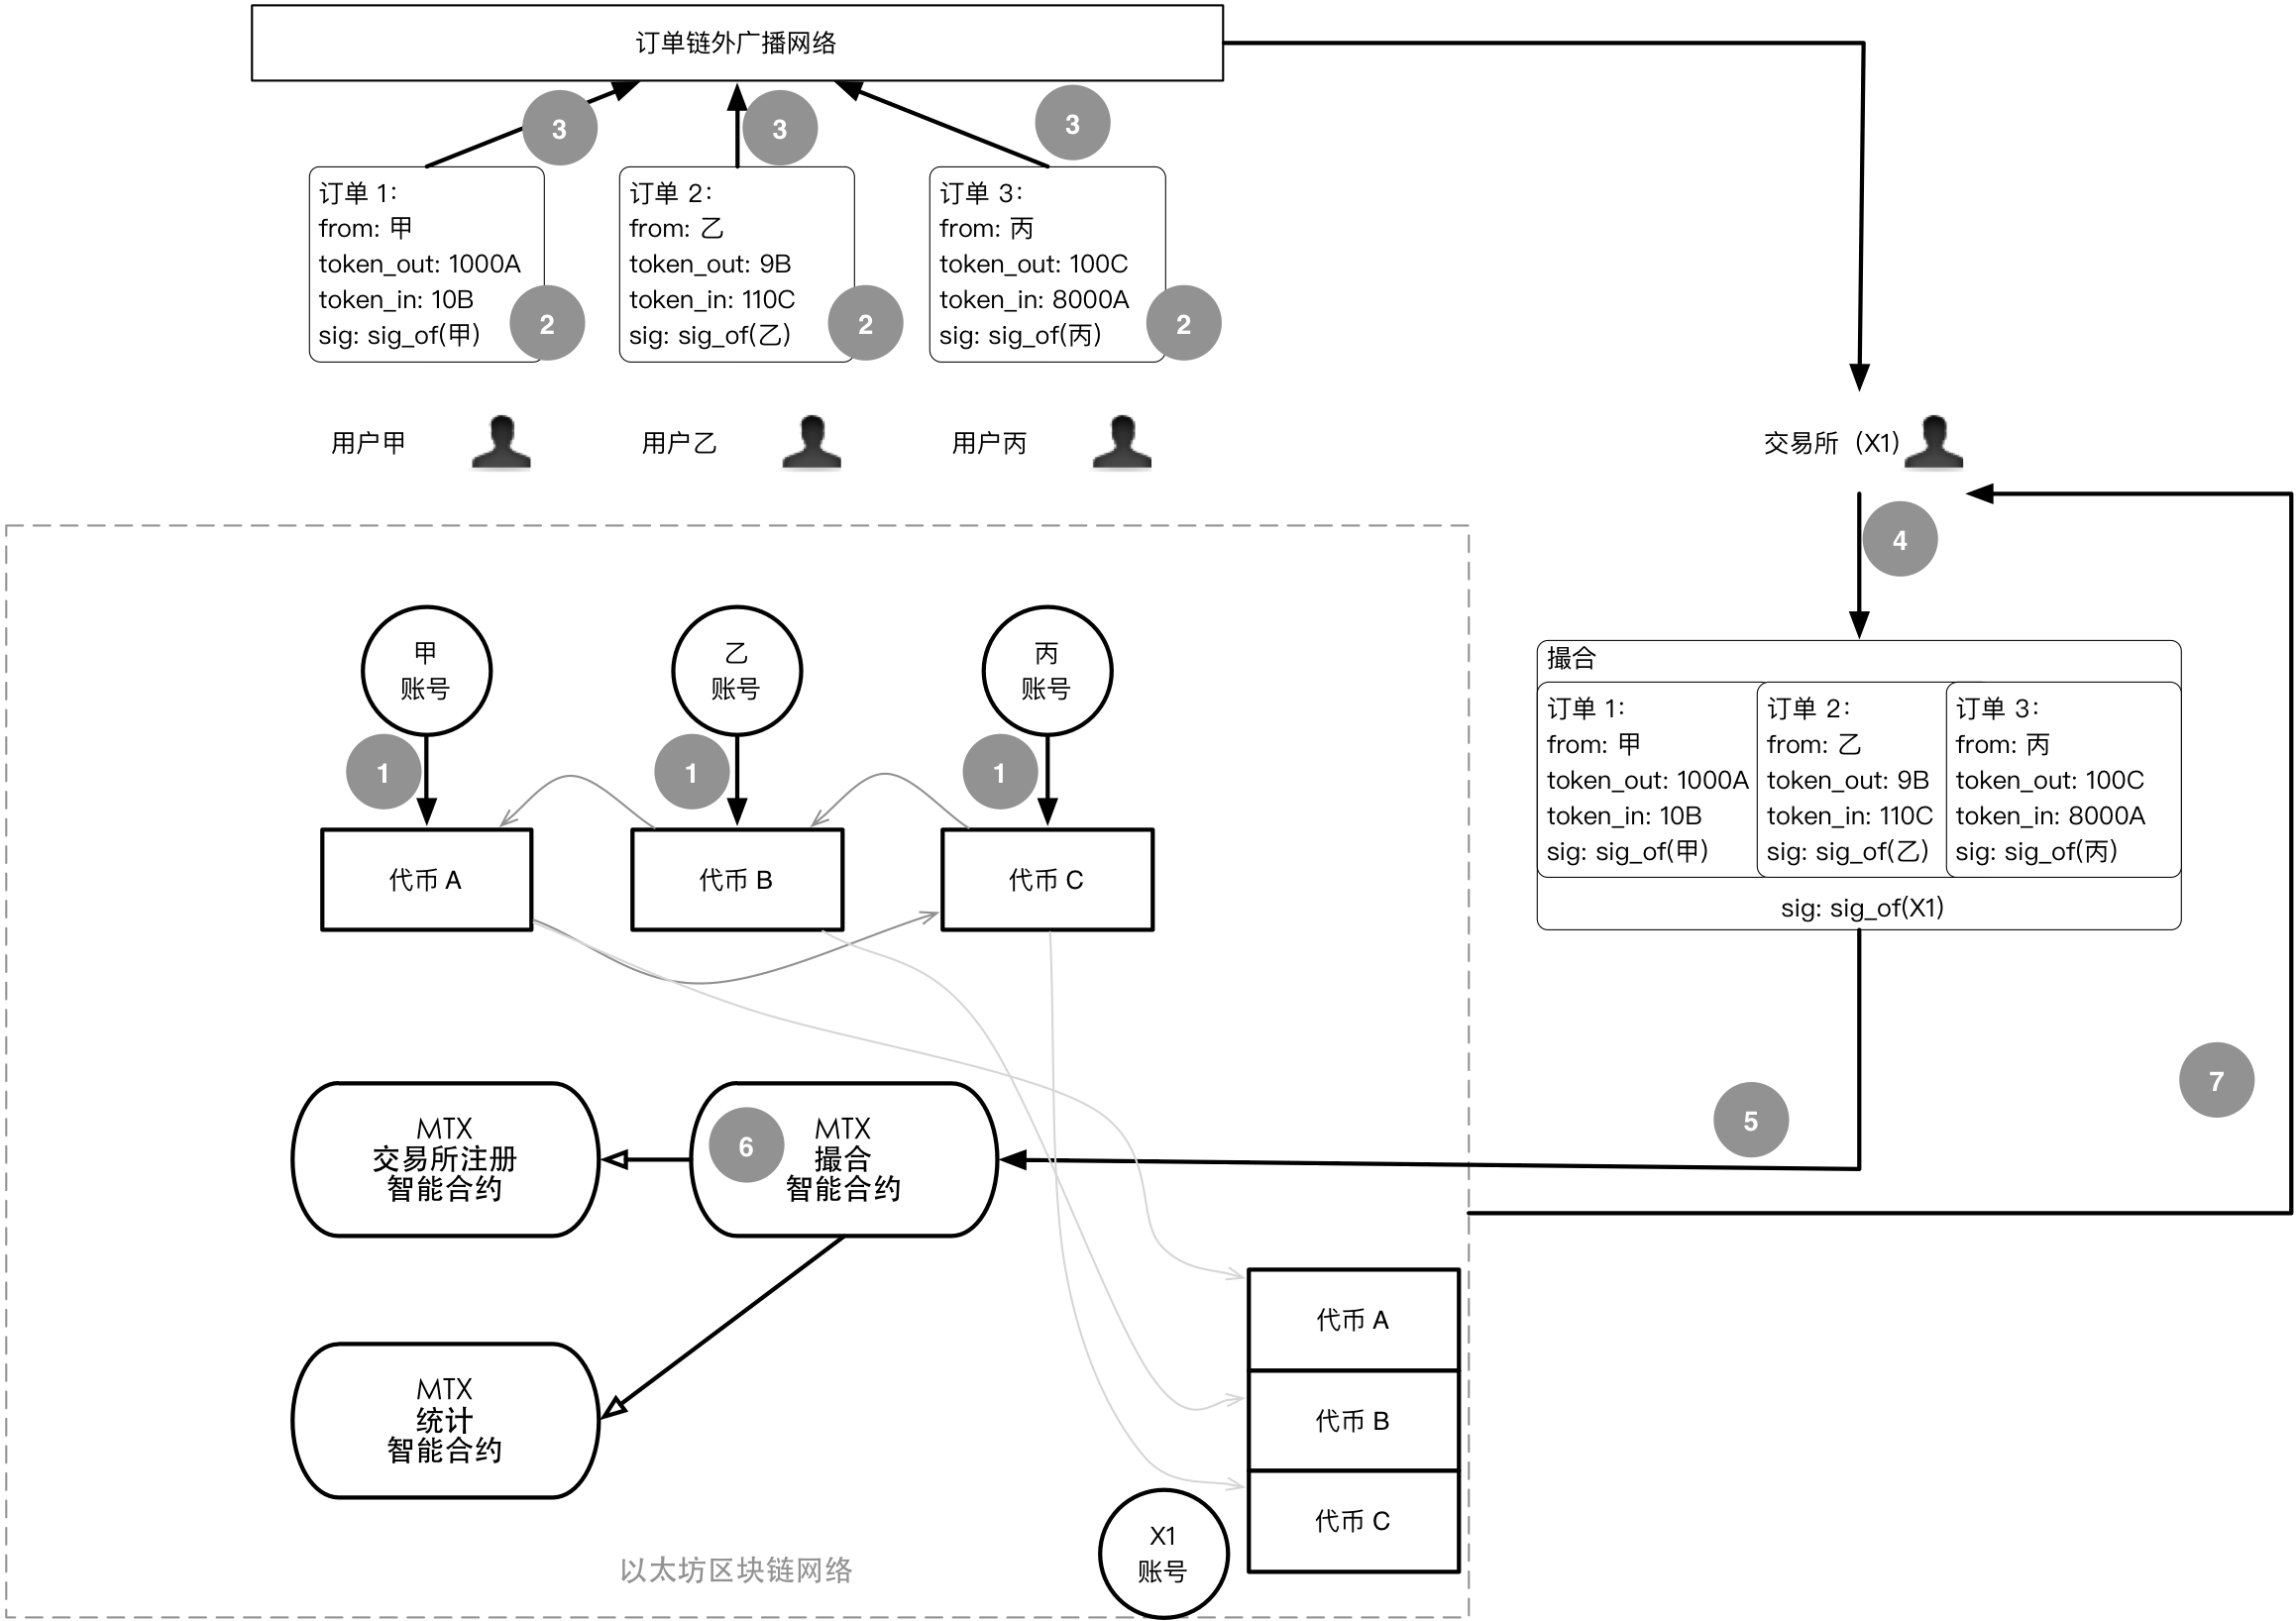
\includegraphics[height=10cm]{images/mtx-protocol.png}
\caption{MTX协议:图中示例一个三边交易的撮合}
\label{fig:mtxprotocol}
\end{figurehere}
\end{center}

采用MTX协议的撮合交易过程如下:

\begin{enumerate}
	\item 用户甲,乙,丙分别对MTX撮合智能合约(Matchengine Contract)授权,授权后该合约可对用户指定代币账号做不超过一定额度的转出操作。在上面实例中,合约可最多从用户甲的账号转出1000个A,从用户乙账户转出9个B,从用户丙账户转出100个C;
	\item 用户甲,乙,丙分别生成自己的订单,并用私钥对其进行数字签名。订单的表示不再区分买单和卖单,所有订单都可以视为是“交换单”: 甲的订单声明:甲愿意支出不多于1000个A,得到尽可能多但不少于10个B;如果是部分成交,那么A到B的兑换率不得低于1000/10,即100.0。订单中还可以包含很多其它的参数,我们在章节\ref{sec:dataformat}中会进一步说明;
	\item 甲,乙,丙分别将自己的订单通过适当的方式广播或定向发送给交易所;
	\item 交易所X1收到上述三个订单,将订单放到三个OrderBook中,并实时通过区块链数据更新订单状态。同时交易所不断计算寻找能够撮合的订单组。一旦确定三个订单的当前状态可以撮合成功,且收益(交易手续费,分润,并去除预估的以太坊gas费)满足预期,则将三个订单组装成一个撮合交易(Match Transaction);
	\item 交易所对撮合交易签名后发送到MTX的撮合智能合约;
	\item 撮合智能合约验证四方签名,之后验证三个订单(的最新状态)是否可以真正成交。若无法成交,合约终止;否则智能合约分别计算出甲乙丙三方各自需要支出的金额,以及交易所X1该收取的费用,并且实时将甲乙丙账号中的资产进行互转,同时支付费用给交易所X1完成清算。在交易过程中,撮合智能合约还会调用MTX注册智能合约(Exchange Registration Contract)来检查交易所是否有权进行撮合,以及费用声明;在交易完成前,还会调用MTX统计智能合约(Trade Stats Contract)对交易所撮合统计做更新,同时更新不同代币间兑换率的变化情况。
	\item 交易所监听新的区块,并根据其中的数据更新相关订单的状态,并根据全部的Orderbook进行新一轮撮合服务。
\end{enumerate}

在传统交易所模型中,被撮合的两方中先下单的为Maker,后下单的为Taker。因为Maker创造流动性而Taker销毁流动性,因此多数交易所的成交价时候会给Maker折扣价,甚至直接采用Maker的价格作为成交价格。与之相比,MTX采用的是All-Maker模型,这是由于在去中心化环境中,很难严格界定哪个单是真正意义上最早的单,因此把所有订单都是被视为Maker既可以简化判断,又可以在计算成交价的时候不偏向任何一方,使得交易更加公平。

MTX协议的另一个显著特点是消除了“交易对(Trading Pair)”的概念。一个从A到B的订单不一定要一个从B到A反向的订单才能撮合,只要有一个交换环路被发现,就可以撮合成功。也可以说传统交易所的市场概念是多边交易闭环的一个最简单的特例。我们后续用订单中两个代币类型的组合来表示订单的类型。

接下类我们介绍可以撮合成交的交易环路的定义和限制,成交价,成交量,和交易所收益模型。为了方便读者理解,我们由一个包含三笔订单的交易环路为例开始,然后引入更一般的情形。


\subsection{订单的归约性}

blahblah


假定有三个币种$A$、$B$和$C$,存在三笔订单:$A\rightarrow B$、$B \rightarrow C$和$C \rightarrow A$,那么就可以形成环路$A\rightarrow B \rightarrow C \rightarrow A$,完成一次跨币种撮合。下面我们对交易环路中的成交价,成交量,和交易所收费做进一步阐述。

\subsection{成交价模型\label{sec:pricemodel}}

令 $P_{A \rightarrow B}$、$P_{B \rightarrow C}$、$P_{C \rightarrow A}$ 分别为这三笔订单的买入价。很容易证明,如果$P_{A \rightarrow B}\cdot P_{B \rightarrow C}\cdot P_{C \rightarrow A}=1$,那么三笔订单恰好可以用各自的买入价完成撮合。当$P_{A \rightarrow B}\cdot P_{B \rightarrow C}\cdot P_{C \rightarrow A}>1$时,可以用低于各自买入价的价格完成撮合,即产生折价。


MTX协议要求交易环路的折价要公平地分摊到每笔订单中。假定三笔订单均得$x\%$的折价,那么最终完成撮合时,三笔订单的成交价分别为:$P_{A \rightarrow B}\cdot (1-x\%)$,$P_{B \rightarrow C}\cdot (1-x\%)$,$P_{C \rightarrow A}\cdot (1-x\%)$。折后价格完成撮合需满足:
\begin{equation}\label{match}
P_{A \rightarrow B}\cdot (1-x\%)\cdot P_{B \rightarrow C}\cdot (1-x\%)\cdot P_{C \rightarrow A}\cdot (1-x\%) = 1\text{,}
\end{equation}
根据上式我们可以推导出
\begin{equation*}
x\%= 1- \frac{1}{\sqrt[3]{P_{A \rightarrow B}\cdot P_{B \rightarrow C}\cdot P_{C \rightarrow A}}}\text{。}
\end{equation*}
在更一般的情形下,如果跨$n$个币种$C_{0}$, …,$C_{n-1}$ 的撮合,那么我们有
\begin{equation*}
x\%= 1- \frac{1}{\sqrt[n]{\prod_{i=0}^{n-1} P_{C_{(i\mod n)} \rightarrow C_{((i+1)\mod n)}}}}\text{。}
\end{equation*}

显然,$\prod_{i=0}^{n-1} P_{C_{(i\mod n)} \rightarrow C_{((i+1)\mod n)}}$ 越大,订单的折价$x\%$越高。因此为了找到具有最高折价的闭环,只需要考虑每个Orderbook中买入价最高的订单。


\subsection{成交量模型}
每个交易环路都是有多个订单组成,而每个订单都会有不同的交易数量,交易数量最小的那个订单会直接影响整个闭环的最终成交数量。当这个交易环路撮合完成后,交易数量最小的这个订单就完全成交了。

假定$A \rightarrow B$、$B \rightarrow C$、$C \rightarrow A$三个订单中,卖出代币的数量分别为$n_{A}$、 $n_{B}$、 $n_{C}$ --- 注意“卖出代币数量并不一定是原始订单中的卖出代币数量,而是订单当前状态的卖出代币数量,参见章节\ref{sec:orderstate} --- 而最终成交的卖出代币数量分别为$N_{A}$、 $N_{B}$、 $N_{C}$。

\begin{theorem}
如果$A \rightarrow B$是三个订单中交易数量最小的,那么$n_{A} = N_{A}$。
\end{theorem}

\begin{proof}
假设$A \rightarrow B$完全成交,那么可以兑换$\frac{n_{A}}{P_{A \rightarrow B}*(1-x\%)}$份额的数字货币B。因此,$B \rightarrow C$可以成交的货币B总金额为

$$N_{B}=\min(n_{B},\frac{n_{A}}{P_{A \rightarrow B}*(1-x\%)})=\frac{n_{A}}{P_{A \rightarrow B}*(1-x\%)}\text{。}$$
同理,$C \rightarrow A$可以成交的货币C 总金额为

\[ \begin{split}
N_{C}&=\min(n_{C},\frac{N_{B}}{P_{B \rightarrow C}*(1-x\%)})\\
&=\frac{n_{A}}{P_{A \rightarrow B}*(1-x\%)*P_{B \rightarrow C}*(1-x\%)}\text{。}
\end{split} \]
同理,$A \rightarrow B$可以成交的货币A总金额为
\[ \begin{split}
N_{A}&=\min(n_{A},\frac{N_{C}}{P_{C \rightarrow A}*(1-x\%)})\\
&=\frac{n_{A}}{P_{A \rightarrow B}*(1-x\%)*P_{B \rightarrow C}*(1-x\%)*P_{C \rightarrow A}*(1-x\%)}\text{。}
\end{split} \]
根据公式\ref{match}可以得出 $N_{A}=n_{A}$。
\end{proof}

\subsection{撮合收益模型}
在整个生态中,负责撮合的交易所处于核心地位。为了鼓励交易所更高效的完成撮合,我们设计了一套针对交易所的经济激励机制。交易所的收入来自两部分:一部分是来自订单的手续费,每一个订单都需要支付一定代币作为手续费,手续费是奖励给交易所的,以激励交易所撮合更多的订单;另一部分是撮合交易环路的利润提成,当交易环路产生利润时,交易所可以按比例从中获得提成,以激励交易所撮合利润更高的交易环路。

如果,交易所上传一个交易环路$C_0 \rightarrow C_1 \rightarrow ... \rightarrow C_{n-1} \rightarrow C_{0}$ 并撮合成功,令每一单$C_{i}\rightarrow C_{(i+1\mod n)}$$(i\in{0,...,n-1})$对应的手续费是$fee_{i}$,那么交易所的手续费收入则为
$
\sum^{n-1}_{i=0}fee_{i}\text{。}
$
交易所的另一部分收入来自于撮合交易的利润提成。如果按照原价每订单$i$够成交$Amt_{i}$,而按撮合后的折价能够成交$Amt'_{i}$,那么交易所就可以从每一单的利润中获得$(Amt'_{i}-Amt_{i})*x\%$的提成,其中$x\%$是提成的比例,因此交易所的撮合交易提成是
$
\sum^{n-1}_{i=0}(Amt'_{i}-Amt_{i})*x\%\text{。}
$
因此交易所的总利润为
$$
\text{总利润} = \sum^{n-1}_{i=0}fee_{i}+(Amt'_{i}-Amt_{i})*x\%\text{。}
$$
交易所在撮合时会综合考虑这两方面的收入做出撮合交易的决策,以优化利润总额。

\subsection{防作弊机制}
我们不允许交易所通过无风险套利窃取闭环的利润,本节我们将介绍如何防止交易所的这种行为。在介绍之前,我们首先来分析交易所如何做到无风险套利。
\begin{definition}[订单的规约]:任何一串跨越$n$个货币的订单$C_{0}\rightarrow C_{1}\rightarrow \cdots \rightarrow C_{n-1}$都可以规约成为一笔订单$C_{0} \rightarrow C_{n-1}$, 那么任何一个交易环路都可以规约到只有两个货币$A$和$B$的$A\rightarrow B\rightarrow A$的环路。令$T_{1} = A\rightarrow B$和$T_{2} = B\rightarrow A$分别为规约后的两笔订单。
\end{definition}

交易所为了自身利益最大化(而不是将折价公平分摊给交易环路上的订单),可以同时生成两个新订单$T'_{1} = B\rightarrow A$和$T'_{2} = A\rightarrow B$,在一个交易环路$<T_{1}$,$T_{2}$,$T'_{1}$,$T'_{2}>$上分别与$T_{1}$ 和$T_{2}$作对冲,使的$x\%==0$,从而让实际成交价变成$T_{1}$和$T_{2}$的买入价。这个环路一个显而易见的特性就是其中包含$<T'_{1}$与$T'_{2}>$这样的子环路。

交易所通过生成带有子环路的撮合,可以实现低风险高收益的回报,从而有效避开协议实际成交价分摊的原则。为了防止这样的套利,我们规定,{\bfseries 合法的闭环必须保证其订单子集无法组成更小的可交易环路}。该要求可以通过以太坊智能合约简单有效地得到验证。当然交易所也可以只对冲其中一笔订单,但是这种对冲方法风险更大,我们会在章节\ref{sec:exchange}中对有交易所的有风险做市行为作进一步探讨。

\subsection{市场深度\label{sec:marketdepth}}

\subsection{数据格式\label{sec:dataformat}}

由于采用All-Maker模型,所有订单都可以用同一个结构表示。该结构包含订单本身的各种参数数据和数字签名。在签名前,现将订单参数数据连接成一个字节数组,通过Keccak SHA3方法对这个字节数组做散列计算得到订单的哈希,之后用账户私钥对这个哈希进行ECDSA签名。


\begin{verbatim}
message Order {
  address protocol;   // MTX协议入口智能合约地址
  address owner;      // 该订单所有者(发起者)地址
  address outToken;   // 卖出ERC20代币智能合约地址
  address inToken;    // 买入ERC20代币智能合约地址
  uint256 outAmount;  // 卖出ERC20代币数量
  uint256 inAmount;   // 买入ERC20代币数量
  unit256 expiration  // 过期时间
  unit256 fee;        // 交易总费用(MTX Token),部分成交的费用按该次匹
                      // 配实际卖出货币额与outAmount比例计算。
  uint8 savingSharePercentage; // fee余额不足时支付给交易所的分润比例
  bytes signature;    // 上面数据的ECDSA签名,也可以用作订单ID
}	
\end{verbatim}

订单中虽然没有明确指定价格,但我们可以通过计算$outAmount/inAmount$来得到一个订单兑换率$P$。该兑换率隐含地要求所有实际撮合成交的兑换率不得大于$P$。一个好的交易所UI应该允许用户指定$outAmount$,$inAmount$,和传统意义的买入价或卖出价这三个数据的任意两个来计算缺失的$outAmount$或$outAmount$值。

订单实际上可以有两种不同的“完全成交”定义:一种定义是只有卖出代币达到了$outAmount$才算完全成交;另一种定义在之前的基础上允许买入代币累计金额达到$inAmount$也算完全成交。我们可以在订单中引入一个参数告诉交易所和撮合智能合约选择哪种完全成交定义。在第一版本的实现中,我们先支持第一种定义。

\begin{verbatim}
message Match {
    Order[] orders;     // 该次匹配的所有订单
    address feeRecipient; // 费用收取地址
    bytes signature;      // 上面数据的ECDSA签名
}
\end{verbatim}

一次撮合中包含的订单应该形成一个可交易环路,并且该环路上同一类型的订单只能有一个 --- 理论上可以将这个限制去掉,不过这会让撮合智能合约更加复杂,因此初期不予支持。放开这个限制的好处是一次撮合中将将更多订单完全成交。



\subsection{订单状态\label{sec:orderstate}}

订单发起者对订单签字广播后无论该订单是否成交,都不会也无法对该订单进行修改,因此撮合智能合约一旦对某个订单进行撮合,就需要就订单的新状态在区块链上更新。对部分或者完全成交的订单,会计算更新$inAmount$和$outAmount$两个值,并且保障订单新状态价格和原始订单的价格一致。如果$inAmount$或$outAmount$为0,则表示该订单已经完全成交。如果用户取消订单,需要发起一个特殊的交易,将$inAmount$和$outAmount$更改为0即可。过期的订单不会触发区块链上的数据更新 --- 可以根据最后一个块的时间戳来判断任何一个订单是否过期 --- 因此我们期待多数的订单会因为过期或者完全成交而变成失效。

交易所需要采用同样的甚至是更复杂的逻辑在区块链外追踪订单状态,尤其是当一家交易监听到到竞争对手在对同一个订单做不同的撮合的时候。我们在章节\ref{sec:exchange}中做进一步探讨。

一个可交易的订单还需要其账户中有足够多的卖出代币余额$balance$,虽然这个余额不要求达到订单中$outAmount$的数量。实际上交易所在对订单状态计算的时候,会取$Max(balance, outAmount)$作为实际的可成交金额。也就是说,交易所不仅仅要监听订单被(其它交易所)撮合的结果,还需要监听订单账户的余额变动情况。看起来这种对区块链数据的监听和对订单状态的更新有些复杂,但这些反而极大简化区块链上合约的逻辑,这种思路和比特币闪电网络,以太坊的雷霆网络的思路是一致的。


\subsection{智能合约\label{sec:contracts}}

MTX协议协议可能包含多个智能合约,包括但不限于:

\subsubsection{撮合合约(Matchengine Contract)} 

该合约计算并确认交易环路中每个订单的状态,计算成交金额和成交量,对交易进行清算转账。给合约还会与其他合约交互,是MTX协议的入口合约。

\subsubsection{订单状态维护合约(Order Contract)}

\subsubsection{交易所注册合约(Registration Contract)}
该合约维护和更新一系列支持MTX协议的交易所,为撮合合约提供交易所预设的参数。这些预设的参数同样也可以节约订单和撮合交易的字节数。

\subsubsection{统计合约(Stats Contract)} 该合约以代币和交易所为对象,计算任何两个币种之间的成交量,成交价,以及不同交易所的贡献度等指标,以及这些指标的某些滑动平均值。这些指标是订单发起者授权撮合的重要参考依据,同时也可以作为某些预测市场的输入,并且为以后可能的协议拓展对条件单进行一定的支持。为了防止交易所经常变动身份,抛弃掉对自己不利的统计数据,MTX协议要求交易所注册时锁定一定额度MTX代币作为信用抵押。我们会在章节\ref{sec:protocoltoken}中做进一步说明。

\subsection{使用ENS\label{sec:registration}}

以太坊提供通过名字解析地址的以太坊名字服务(Ethereum Name Service, ENS)\cite{hirai2016formal}。我们可以通过使用ENS,将MTX协议中所有的智能合约,ERC20代币发行地址,交易所收益地址等地址信息映射到相应的名字,一方面可以降低订单信息出错的可能性,另一方面也会减小订单和撮合交易的字节数。


这些合约的具体实现需根据以太坊智能合约语言的限制做适当修改,不排除将上述合约进一步拆解或合并的可能。

值得指出,这些智能合约是完全开放的,这意味着它们可以被任何的dApp直接或者间接调用。因此整个协议即使一个完善的整体,又是个开放的,单独可用的组件的集合。

\section{MTX协议代币\label{sec:protocoltoken}}



[段落:代币用于支付交易费,更节约成本]

[段落:交易所购买代币进行注册的抵押]

[段落:协议代币也是ERC20,可以同样方式交易,因此生态是个完整闭环]


\section{交易所\label{sec:exchange}}

交易所为用户提供的核心价值是价格发现和交易撮合。交易所的价格发现服务通过汇聚尽可能多的订单,并且对订单进行状态追踪和更新,按照兑换率排序形成多个全局的多Orderbook,同时根据多个Orderbook,计算出任何两个代币之间的兑换率历史和特定的统计指标,比如最新兑换率,滑动成交趋势等等。交易撮合服务建立在价格发现服务的基础之上,通过优化多边交易环路发现算法,尽可能快地将撮合提交到以太坊区块链,通过智能合约做撮合验证和清算。我们预测交易所的第三个重要服务是代币发行和承兑服务,将以太坊链外资产引入到以太坊网络。不过这个服务和本文的协议相关性不大,我们不做进一步阐释。

交易所撮合服务的收入是撮合手续费或分润。订单中可以指定一个$fee$,这是该订单在完全成交后愿意支付给交易所的费用 --- 以协议代币计价。如果订单是部分成交,则按照相应比例支付$fee$的一部分给交易所。如果该订单拥有者账户中用于支付该次撮合的协议代币不足,撮合智能合约会通过分润的计算来支付订单中的一部分卖出货币给交易所。

交易所并不能保证每一个撮合都是盈利的。一方面的原因可能是成本过高,因为交易所为了激励旷工有限打包自己的撮合交易到区块链,因此可能根据预期的收益调高gas,这部分gas是用以太计费的,而以太和撮合中代币的价格相对价格有可能有交大浮动,从而造成gas实际成本更好。另一方面的原因是收入没有达到预期,比如交易所把撮合广播到区块链后,该撮合的某个订单的卖出货币被部分或者全部转移到另一个地址,从而造成整个撮合交易不被智能合约接受。类似这样的原因还有很多,因此交易所的每次撮合广播都是根据自己的经验和算法,最大化长期利益的概率游戏。不过也不用担心,实际上交易所和订单发起者是双向选择的关系:交易所只会选择有利可图的订单;而订单发起者只会选择撮合速度最快,撮合价格最理想的交易所 --- 这是通过MTX的统计合约数据得到支撑的。

[段落:价值,收入,相互竞争,交易所时间和利润的平衡,旷工对撮合的选择和利益]

[段落:交易所评分]

[段落:交易所如何实现短期利润最大化]

[段落:交易所的信用积累]

%[段落:交易所的初创成本]


[段落:如何激励转发订单???]


\section{ICO\label{sec:ico}}

我们计划发行1亿 MTX代币,8千万发给众售收参与者,2千万有MTX开源项目委员会掌管,服务于众售营销,社区维护,员工增长和未来5年的发展需要。

项目预期将于2017年第四季度开启前期投资人的ICO和对市场公开的ICO。目标融资金额分别为3000万人民币和5000人民币等值的ETH。筹集的ETH将按照众筹方案发行出MTX平台的代币MTX.所有众售得来的ETH资金都由MTX开源项目委员会负责支出。初期的支出计划如下:

\begin{table}[hbt]
  \centering
  \begin{tabular}{l|c}
 用途   & 占比\\
    \hline
  技术研发 & 50\% \\
  社区建设 & 20\% \\
  市场推广 & 15\% \\
  专利、法务等 & 15\% \\
  \end{tabular}
  \caption{支出计划}
\end{table}


项目的众售和研发时间表
\begin{table}[hbt]
  \centering
  \begin{tabular}{l|l}
 时间   & 目标\\
    \hline
  2017年6月 & 白皮书发布,项目启动 \\
  2017年7月 & 原型开发完成 \\
  2017年8月 & MTX开源项目委员会(基金)成立并完成私募 \\
  2017年8月 & 公开ICO计划 \\
  2017年9月 & ICO启动 \\
  2017年10月 & ICO结束并公开结果 \\
  2017年11月 & 交易所MTX代币IOU交易开启 \\
  2017年12月 & 上线公测 \\
  2018年2月 & 正式上线 \\
  \end{tabular}
  \caption{项目时间表}
\end{table}

\subsection{代币在ETH和ETC双链发行\label{sec:chains}}

虽然我们只支持通过ETH众筹,但我们也意识到ETC作为智能合约平台的潜力。因此我们会同时在Ethereum(ETH)和Ethereum Classic(ETC)两条链上同时为众筹的地址发行MTX代币。我们不接受ETC众筹的原因主要是因为无法简单有效对两种资产做兑换率计算,进而可能会产生代币分配的不公。


\subsection{风险提示\label{sec:risks}}

ICO作为一种新的众筹模式,存在着各种不同的风险,参与ICO需要充分意识到这些风险:
\begin{itemize}
	\item MTX代币不赋予控制权 - 控制MTX代币不能赋予其控制人对MTX平台或任何关联企业的所有权或股权。MTX代币不赋予任何参与涉及MTX平台的决策的权利。
	\item 不保证营销带来的收益或利润 - 此文中所有的收益和利润举例仅为展示目的,或代表行业平均值,并不构成对营销结果的保证。
	\item 监管不确定性 - 区块链相关的科技已经成为全世界不同监管机构的监管和审查目标。MTX代币网络可能会受到一个或多个监管调查或行为的冲击,包括但不限于对MTX这样的电子代币的使用或持有的限制,这可能损害或限制MTX代币未来的功能和回购操作。
	\item MTX代币不是投资品 - MTX代币不代表任何正式或有法律约束力的投资品。鉴于不可预知的情况,本白皮书列出的目标可能发生变化。虽然我们会尽力实现本白皮书的所有目标,所有购买MTX代币的个人和团体因此将自担风险。
	\item 丢失风险 - 来自众售的资金未获得保险。如果发生丢失事件,或价值损失,将没有公共或私营保险人会提供给购买者保障。
	\item 与MTX开发人员雇主公司无关 - MTX代币的众售资金并不由任何与相关开发人员的雇主相关或所有。MTX开源项目委员会独立实体,有着完全独立的所有权结构。
	\item 失败风险 - 有可能发生的是,由于任何可能的原因,包括但不限于商业关系或营销战略的失败,MTX平台和所有的众售资金支持的后续营销将不能取得成功。
	\item 免责声明 - 你同意,你使用或不能使用MTX代币都由你自己承担风险,且不追究MTX开源项目委员会的责任。初次发行后,MTX代币将被发送给你,但不附加任何形式的保证,无论是明确表达还是暗示的,包括所有暗示的可销售性保证、对特定目的的契合、头衔和非侵权性。由于某些司法辖区不允许不包含暗示性保证,上述不包含暗示性保证的表述可能不适用于你。
\end{itemize}


\section{鸣谢\label{sec:acknowledgement}}

\bibliography{whitepaper}
\bibliographystyle{acm}

\end{document} 